\indent Veremos que es lo que sucede al ir variando los parámetros de entrada para cada familia, de manera tal que, a medida que F, C y P crecen linealmente podamos observar que sucede con cada familia de casos (es decir, las familias se mantienen, solo varia el tamaño de la entrada en todos los casos).\\
Se comienza, por lo tanto, con una entrada de 5 filas y columnas y se la aumenta en cada test en una fila y columna hasta llegar a una matriz de 50*50. De manera que no hay desigualdades y todas las familias se miden en instancias de igual tamaño.\\
El origen siempre estará en la primer columna posible y el destino en la última. A medida que la matriz crezca, las posiciones de los mismos no serán alteradas y la cantidad de paredes y como varie el $P_{max}$ en cada caso, serán acordes para que siempre se encuentren dentro de la misma familia.

Para obtener dichas instancias se realizaron aproximadamente unas 20 corridas con el mismo input y se tom\'o el promedio de las mismas en cada instancia para obtener un valor m\'as cercano a la media.\\ 



Se puede observar en el  gráfico 1.1, cinco funciones, que representan el tiempo de ejecuci\'on de las familias de casos mencionadas en el apartado anterior:\\

\begin{enumerate}
\item No existe camino para atravezar el laberinto
\item Existe un camino sin atravesar paredes para recorrer todo el laberinto
\item Rompiendo todas las paredes posibles para pasar el laberinto
\item Rompiendo una cantidad menor de paredes posibles para pasar el laberinto
\item Múltiples caminos para llegar a destino
\end{enumerate}

\vspace*{0.3cm} \vspace*{0.3cm}
  \begin{center}
 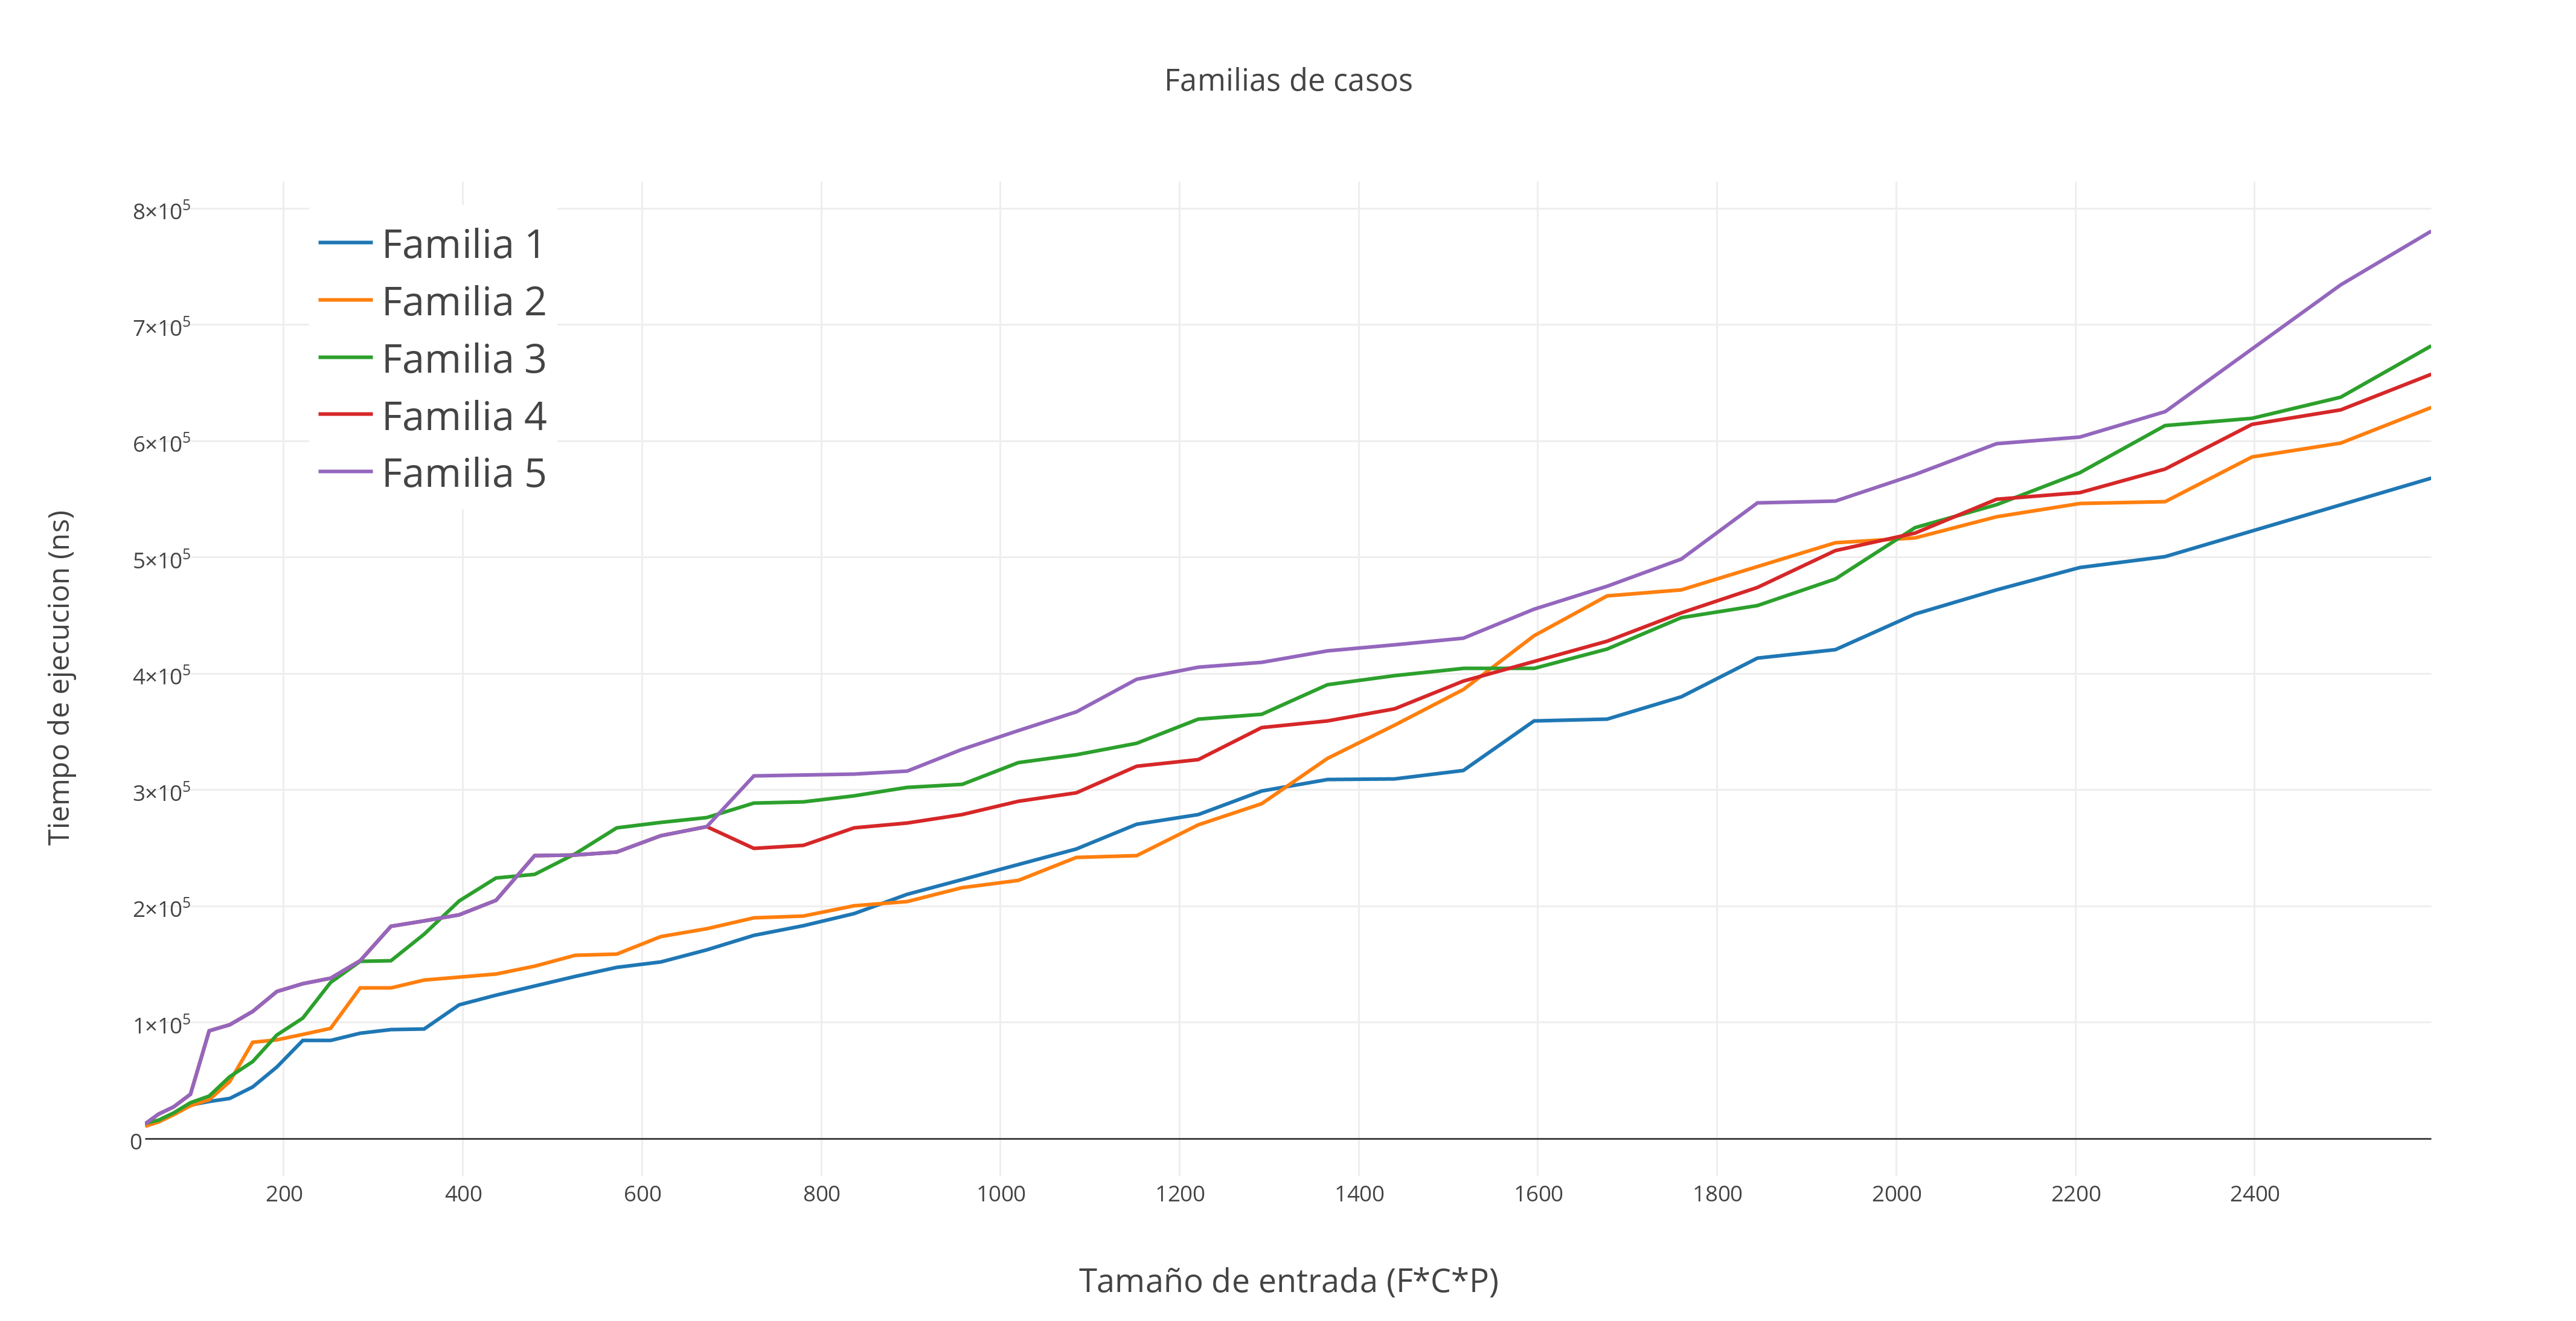
\includegraphics[scale=0.5]{./EJ1/comparativo.png}
 {Gr\'afico \ 1.1 - $Comparativo$}
  \end{center}
  \vspace*{0.3cm}
  
Se puede notar que la familia 1 "\textbf{No existe camino para atravezar el laberinto}", presenta una mejor performance en relaci\'on a las otras. Esto se puede deber a dos motivos, o bien en el primer paso no puede salir por ning\'un camino posible o bien su adyacente es el nodo destino, por lo tanto chequea solo los nodos adyacentes al origen y finaliza su ejecuci\'on. Con lo cual esta familia representa el mejor caso en performance para el algoritmo.

\vspace*{0.3cm} \vspace*{0.3cm}
  \begin{center}
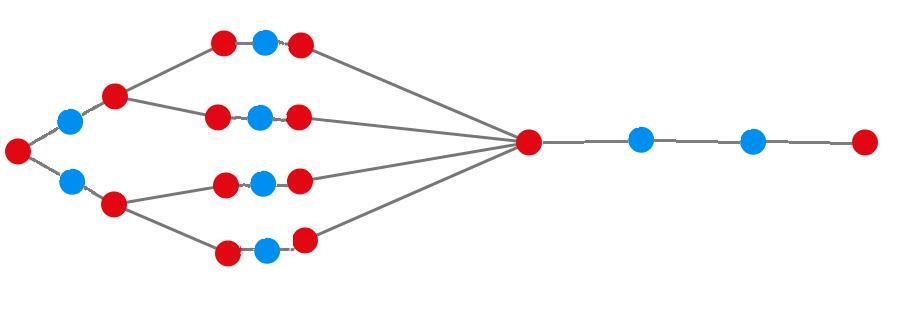
\includegraphics[scale=0.7]{./EJ1/ej1grafomejorcaso.jpeg}
{Grafo 1.1 - $Con$ $P=0$ Termina sin poder romper paredes en una iteracion}
  \end{center}
  \vspace*{0.3cm}

\vspace*{0.3cm} \vspace*{0.3cm}
  \begin{center}
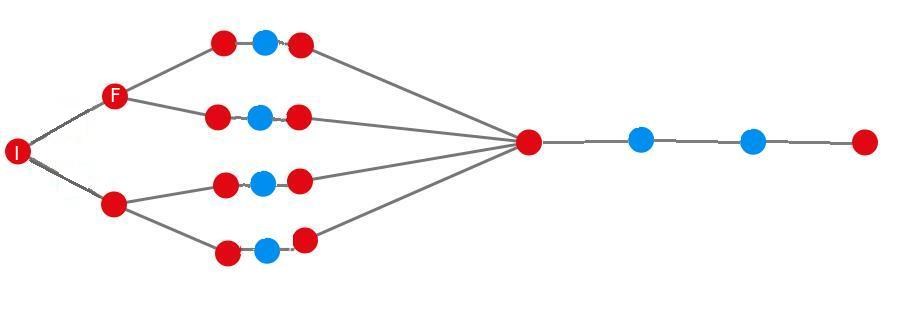
\includegraphics[scale=0.7]{./EJ1/ej1grafomejorcaso2.jpeg}
{Grafo 1.1 - $Con$ $P=0$ Nodo destino (f) vecino a nodo inicio (i)}
  \end{center}
  \vspace*{0.3cm}

Uno de los peores casos para nuestro algoritmo es la familia 5 "\textbf{Múltiples caminos para llegar a destino}", que sucede cuando por ejemplo, todos los caminos tienen igual longitud. Esto se da as\'i ya que nuestro algoritmo chequea todos los caminos posibles y como todos pueden ser soluci\'on posible avanza por todos y llega al final del laberinto con el mismo valor en todos los posibles caminos.\\

\vspace*{0.3cm} \vspace*{0.3cm}
  \begin{center}
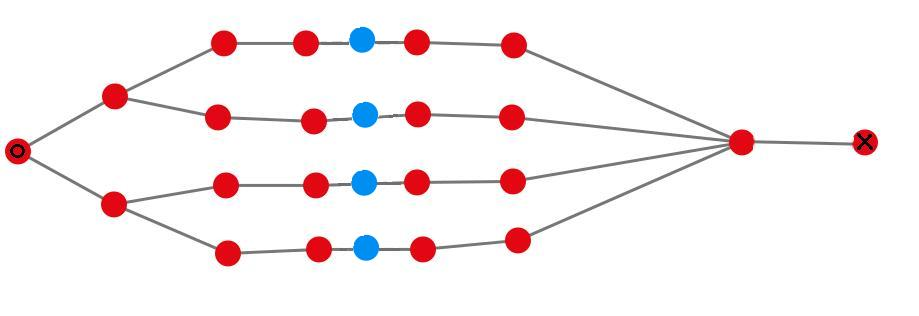
\includegraphics[scale=0.7]{./EJ1/ej1grafopeorcaso.jpeg}
{Gr\'afico 1.2 - Múltiples caminos para llegar a destino de misma longitud}
  \end{center}
  \vspace*{0.3cm}

\textit{---> habria que explicar un poco que pasa en los otros casos!!!}\\

Veamos en detalle como se comportan el mejor y peor caso con respecto a la complejidad calculada.\\

  \vspace*{0.3cm} \vspace*{0.3cm}
  \begin{center}
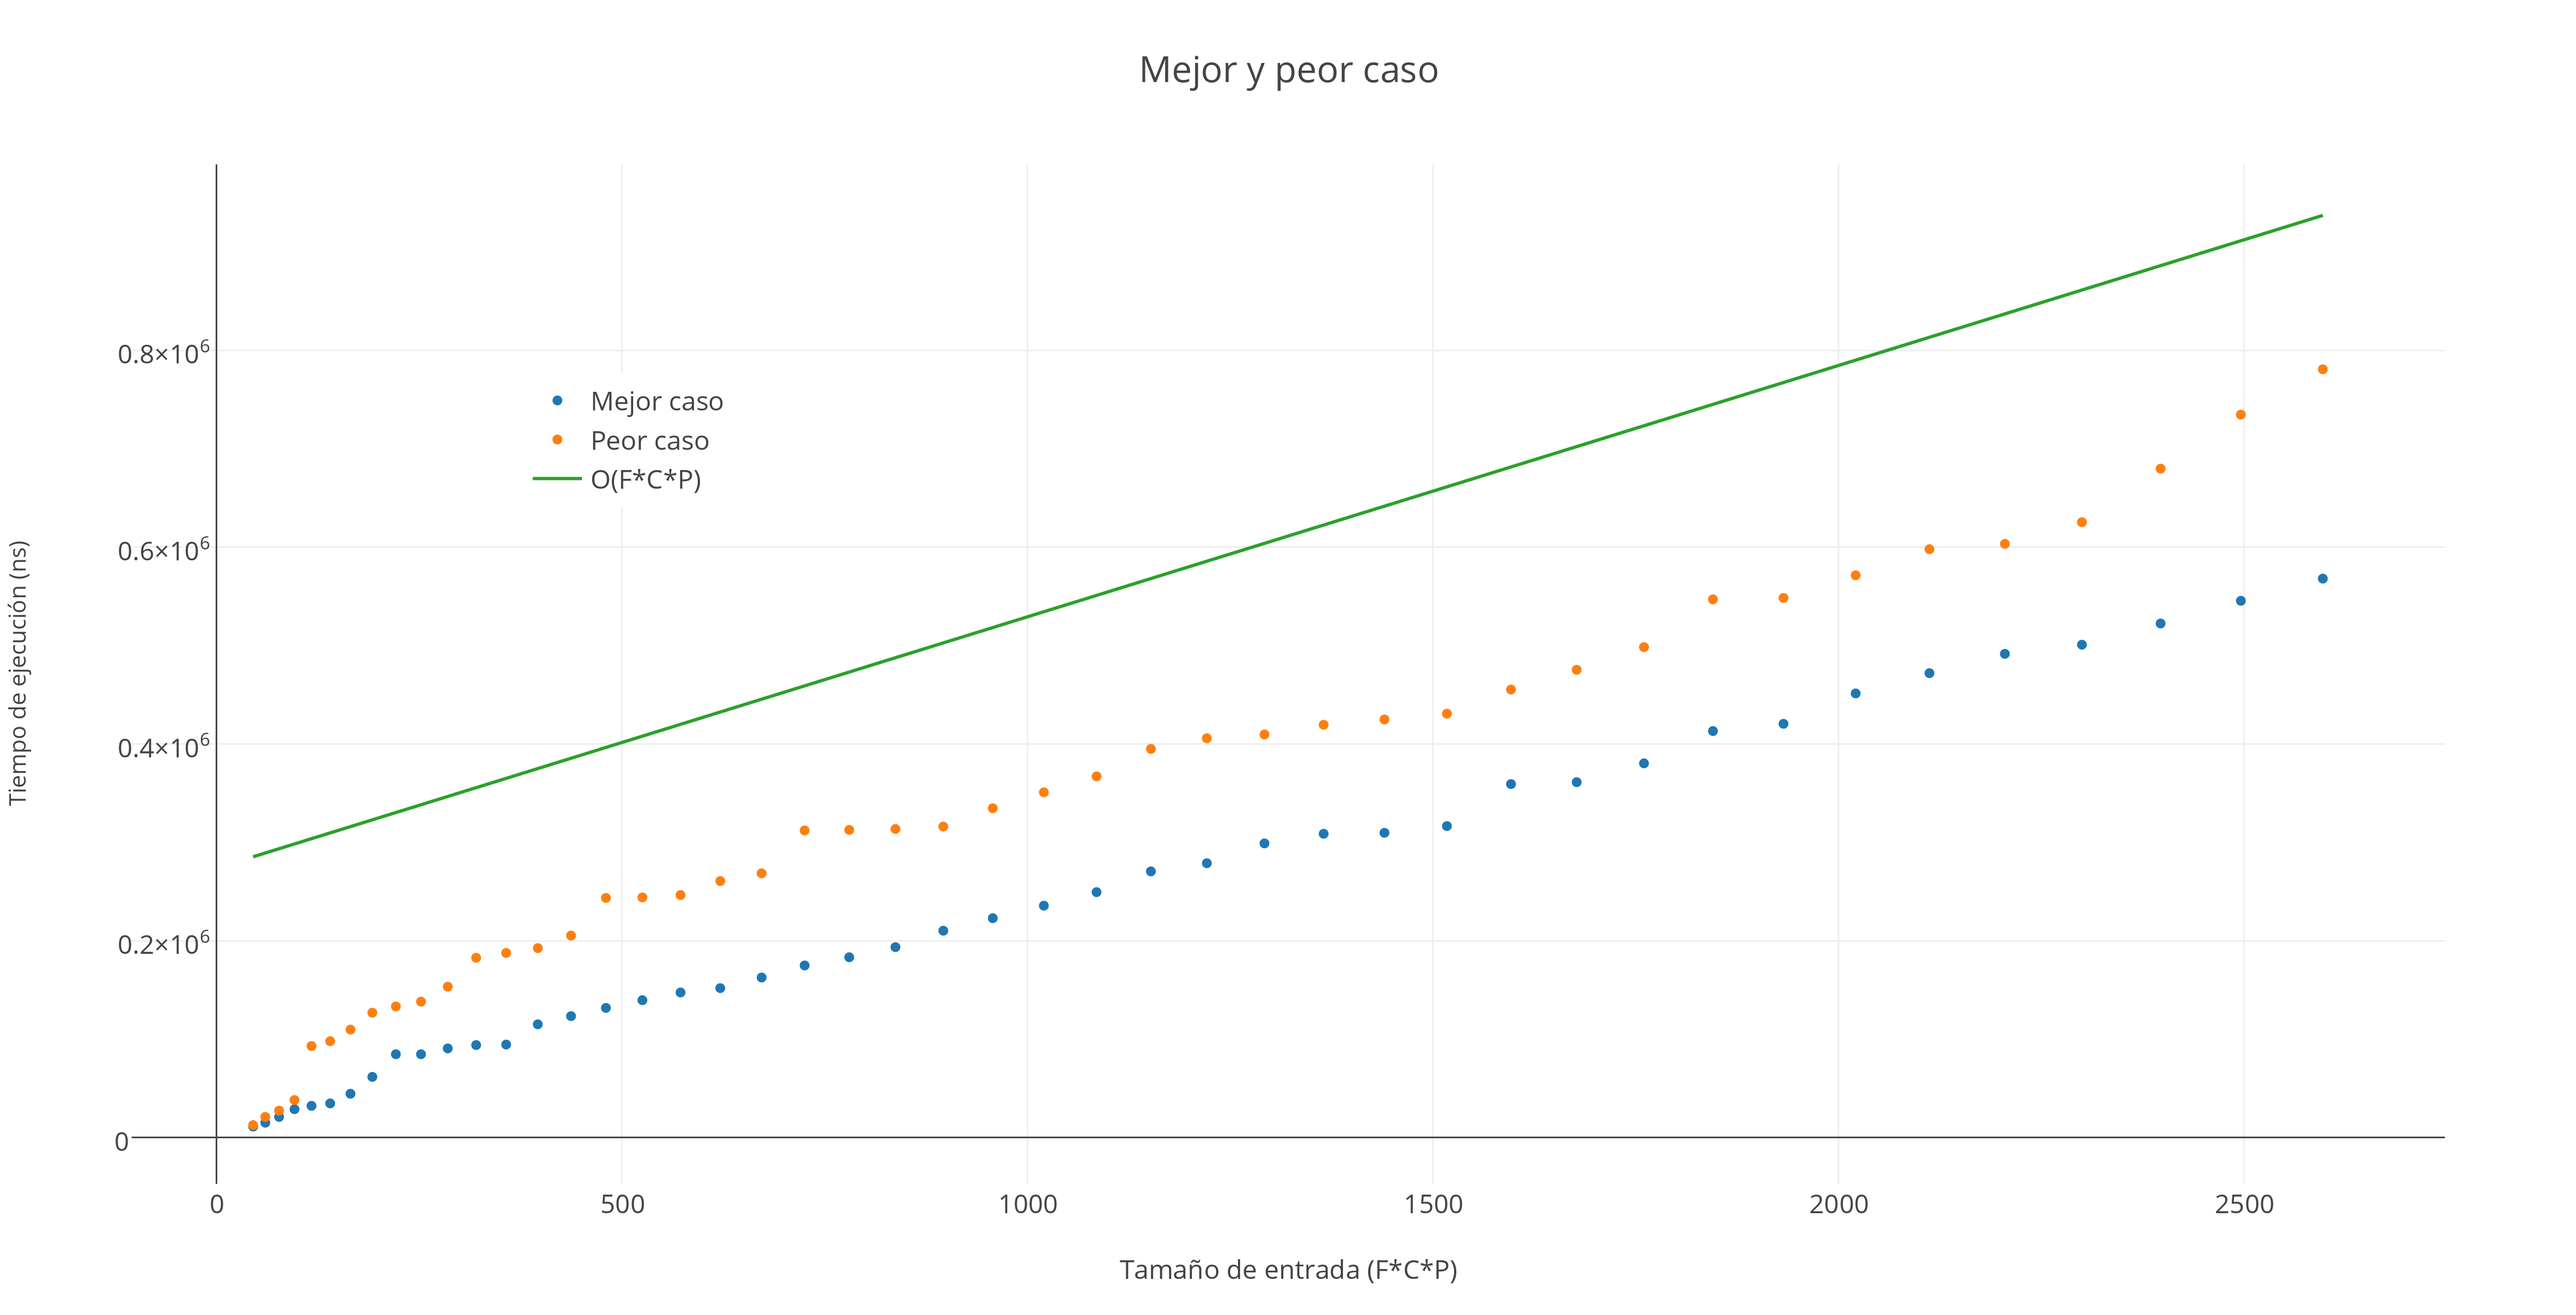
\includegraphics[scale=0.5]{./EJ1/MejorYPeorCaso.png}
{Gr\'afico 1.5 - $Comparativo$}
  \end{center}
  \vspace*{0.3cm}
  
Podemos ver en este gr\'afico comparativo como las familias est\'an acotadas por la funci\'on de la complejidad te\'orica calculada.\\

\textit{---> Sobre la complejidad teorica calculada habria que decir algo no? porque F*C*P parece una cubica? habria que hablar un poco de que a P tenes que aumentarlo casi linealmente junto con el tamaño de F y C. El test del final creo que quiere mostrar un poco eso, aunque para mi esta mal. La idea es decir que no sirve de nada fijar el tamaño de la matriz o fijar P porque no genera resultados que muestren algo sobre el algoritmo, y que por eso al final tus resultados son cubicos, tenes tres variables aumentando casi linealmente y con valores parecidos, por eso termina estando dentro de la familia de las cubicas}\\
\textit{---> Lo que decis aca esta mal, el mejor y peor caso NUNCA van a tener la misma cantidad de paredes sino se comportarian igual}

Mostraremos a continuaci\'on sobre un grafo de tamano fijo, es decir, F y C no variables ambos en 50 y con P variable, que es lo que sucede al ir agregando linealmente una cantidad de paredes determinada entre el nodo inicio y destino de manera que...??\\

\textit{---> De manera que??? pensa que es lineal para este grafo que armaste que ni siquiera explicaste como es...que es lo que pasa cuando agregas paredes? En la conclusion hablas de que se hacen O(P) operaciones...porque? porque voy a necesitar chequear todas las paredes? capas ni hace falta...pensa en el mejor caso. Si agregas paredes y paredes del lado donde no esta el nodo final no influye!! Si queres decir que sucede para cualquier grafo...entonces tenes que MOSTRARLO!}\\

\textit{--->Esto no lo puse yo, solo puse que se iba a ver q pasaba y despues sacaba una conclusion que si o si tiene q ser lineal ya que el tamño de entrada es FIJO osea 50*50 y como solo se va modificando la cantidad de paredes que podes romper se mantiene lineal si o si y va a ir variando siempre}


\vspace*{0.3cm} \vspace*{0.3cm}
  \begin{center}
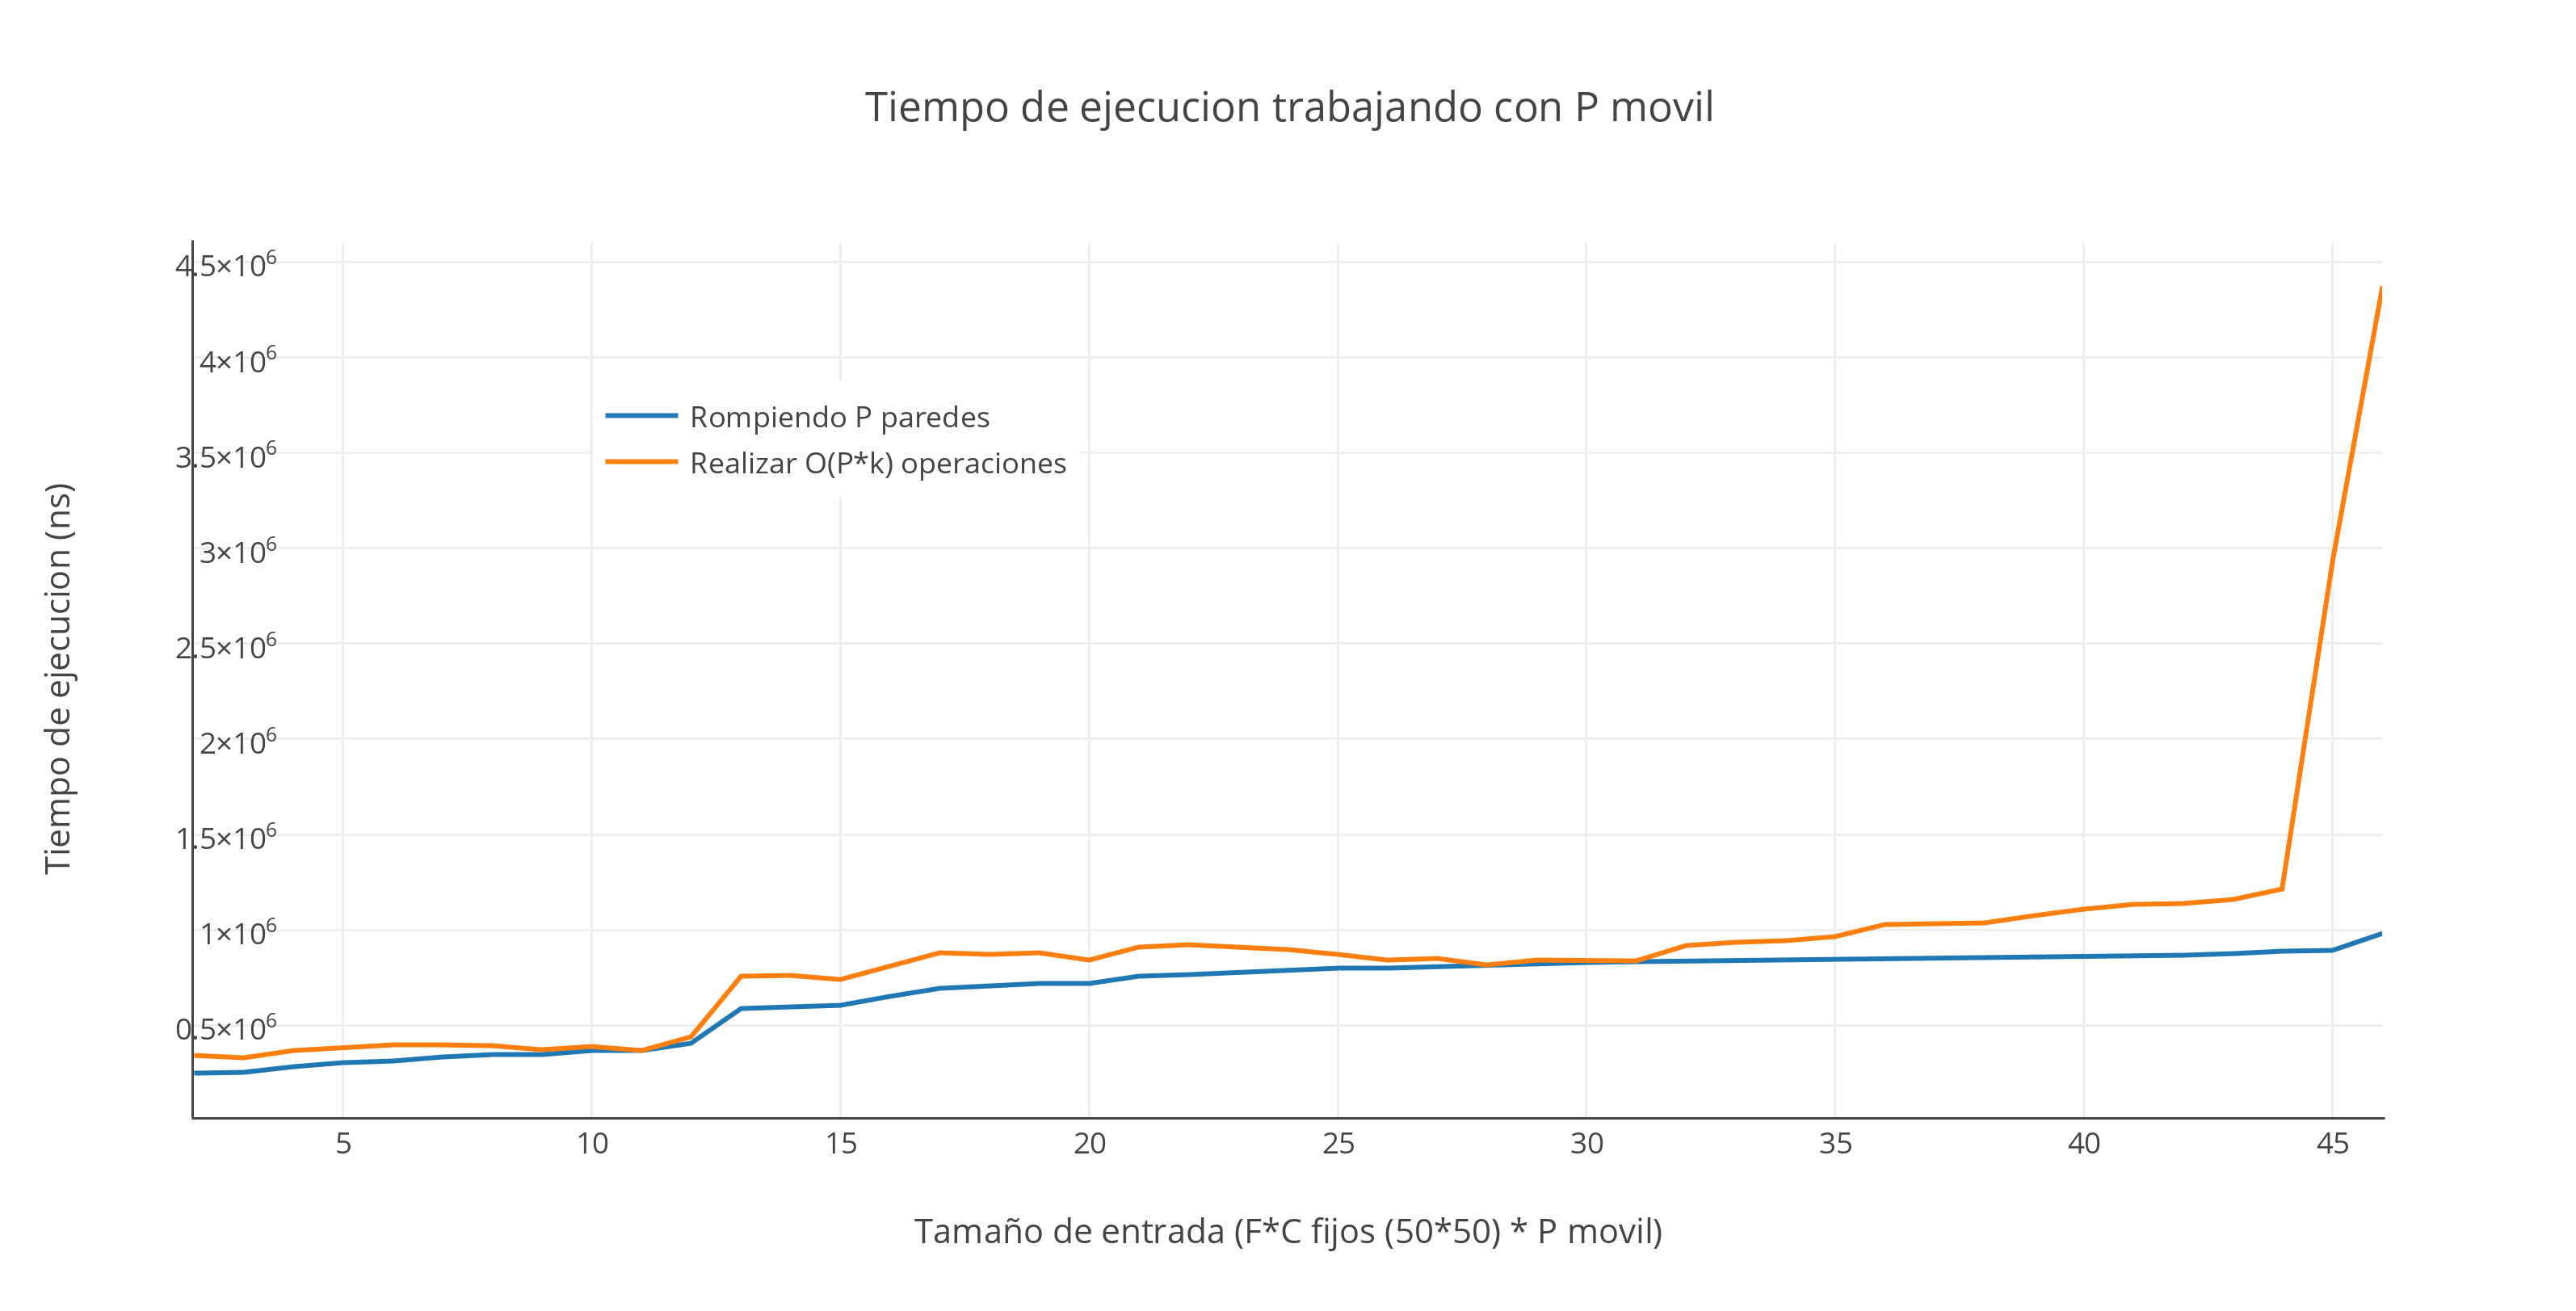
\includegraphics[scale=0.7]{./EJ1/pVariable.png}
{Gr\'afico 1.6 - $P$ $variable$ $y$ $F,C$ $fijos$}
  \end{center}
  \vspace*{0.3cm}

Se puede observar en el gr\'afico 1.6 como al aumentar P, aumenta linealmente el tiempo de resoluci\'on, ya que se agrega una cantidad extra de paredes manteniendo la cantidad de nodos del grafo. Se chequea por lo tanto que trabajar con una cantidad fija de nodos nuestro algoritmo realiza O(P) operaciones por cada elemento del grafo.\\

\textit{---> Otra vez, como sabes que es lineal?, es mas, hasta parece constante. Para empezar esta mal explicado el experimento. Pensa que Curcio nos dijo en general que los experiementos tenian las conclusiones flojas y esto yo lo escuche!}\\

Luego de lo mostrado, se pudo observar que, tanto en el mejor como en el peor caso nuestro algoritmo se encuentra en el orden de la complejidad calculada.
